\begin{figure}[t]
\centering
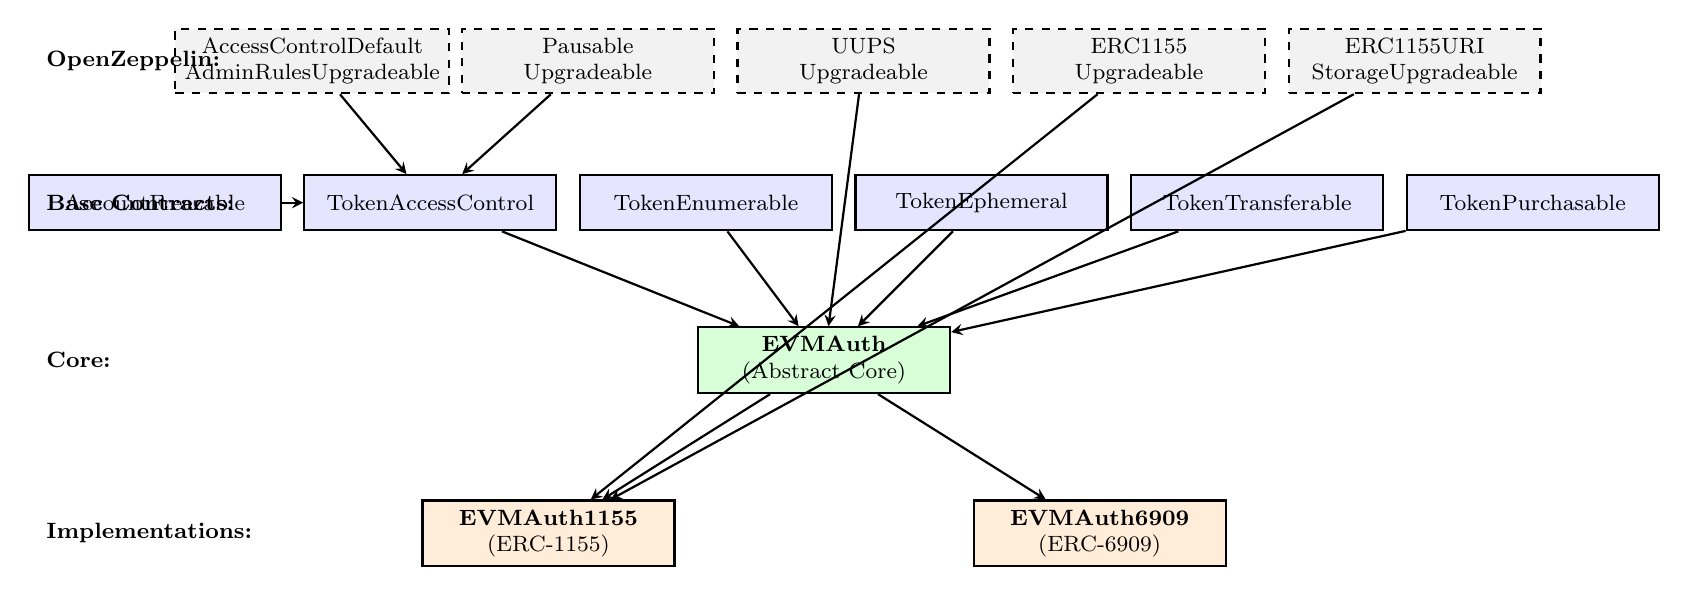
\begin{tikzpicture}[
    base/.style={rectangle, draw, thick, minimum width=3.2cm, minimum height=0.7cm, align=center, fill=blue!10, font=\footnotesize},
    core/.style={rectangle, draw, thick, minimum width=3.2cm, minimum height=0.7cm, align=center, fill=green!15, font=\footnotesize},
    impl/.style={rectangle, draw, thick, minimum width=3.2cm, minimum height=0.7cm, align=center, fill=orange!15, font=\footnotesize},
    oz/.style={rectangle, draw, thick, dashed, minimum width=3.2cm, minimum height=0.7cm, align=center, fill=gray!10, font=\footnotesize},
    arrow/.style={->,>=stealth,thick}
]

% OpenZeppelin Base Contracts (Top Layer - Dashed)
\node[oz] (ozaccess) at (0,6) {AccessControlDefault\\AdminRulesUpgradeable};
\node[oz] (ozpause) at (3.5,6) {Pausable\\Upgradeable};
\node[oz] (ozuups) at (7,6) {UUPS\\Upgradeable};
\node[oz] (oz1155) at (10.5,6) {ERC1155\\Upgradeable};
\node[oz] (oz1155uri) at (14,6) {ERC1155URI\\StorageUpgradeable};

% Base Contracts Layer (Second Layer)
\node[base] (accfreeze) at (-2,4.2) {AccountFreezable};
\node[base] (acccontrol) at (1.5,4.2) {TokenAccessControl};
\node[base] (enumerate) at (5,4.2) {TokenEnumerable};
\node[base] (ephemeral) at (8.5,4.2) {TokenEphemeral};
\node[base] (transfer) at (12,4.2) {TokenTransferable};
\node[base] (purchase) at (15.5,4.2) {TokenPurchasable};

% Core Layer (Third Layer)
\node[core] (evmauth) at (6.5,2.2) {\textbf{EVMAuth}\\(Abstract Core)};

% Implementation Layer (Bottom Layer)
\node[impl] (evm1155) at (3,0) {\textbf{EVMAuth1155}\\(ERC-1155)};
\node[impl] (evm6909) at (10,0) {\textbf{EVMAuth6909}\\(ERC-6909)};

% Inheritance Arrows - OpenZeppelin to Base Contracts
\draw[arrow] (ozaccess) -- (acccontrol);
\draw[arrow] (ozpause) -- (acccontrol);
\draw[arrow] (accfreeze) -- (acccontrol);

% Inheritance Arrows - Base Contracts to EVMAuth Core
\draw[arrow] (acccontrol) -- (evmauth);
\draw[arrow] (enumerate) -- (evmauth);
\draw[arrow] (ephemeral) -- (evmauth);
\draw[arrow] (transfer) -- (evmauth);
\draw[arrow] (purchase) -- (evmauth);
\draw[arrow] (ozuups) -- (evmauth);

% Inheritance Arrows - EVMAuth to Implementations
\draw[arrow] (evmauth) -- (evm1155);
\draw[arrow] (evmauth) -- (evm6909);

% Inheritance Arrows - OpenZeppelin to ERC-1155 Implementation
\draw[arrow] (oz1155) -- (evm1155);
\draw[arrow] (oz1155uri) -- (evm1155);

% Layer Labels
\node[anchor=west, font=\footnotesize\bfseries] at (-3.5,6) {OpenZeppelin:};
\node[anchor=west, font=\footnotesize\bfseries] at (-3.5,4.2) {Base Contracts:};
\node[anchor=west, font=\footnotesize\bfseries] at (-3.5,2.2) {Core:};
\node[anchor=west, font=\footnotesize\bfseries] at (-3.5,0) {Implementations:};

\end{tikzpicture}
\caption{EVMAuth contract inheritance hierarchy. Base contracts (blue) provide orthogonal authorization primitives. EVMAuth core (green) coordinates all primitives into a unified interface. Implementations (orange) integrate token standards (ERC-1155 or ERC-6909) with EVMAuth primitives. Dashed boxes represent OpenZeppelin dependencies.}
\label{fig:contract-hierarchy}
\end{figure}
